\section{Results}
\label{sec:results}

All numbers in this section are held-out results.
agent-ho, gcsn-ho and the sweep are \emph{previously examined} on every CPU (Section~\ref{sec:workload}); the BEIR sets are fresh.
Ratios are rival / \sweet; above 1 means \sweet is faster.
The EPYC (Zen~3) rows are still to come \TODO{epyc}.

\subsection{Warm calls, all cores}
\label{sec:warm}

Table~\ref{tab:warm} and Figure~\ref{fig:ratios} give the main comparison.
Against the exact rivals with float32 inputs, \sweet was faster on every CPU and on all three replayed workloads.
The fastest such rival needed \nm{best.warm.agent-ho.f32.min}--\nm{best.warm.agent-ho.f32.max}$\times$ the time on agent calls, \nm{best.warm.gcsn-ho.f32.min}--\nm{best.warm.gcsn-ho.f32.max}$\times$ on GCSN calls and \nm{best.warm.beir.f32.min}--\nm{best.warm.beir.f32.max}$\times$ on BEIR calls.
Which rival came closest depends on the CPU: PyTorch on Intel and AMD agent calls, NumPy on Graviton4 and the M3 Max, maxsim-cpu on Intel BEIR calls, and NextPlaid on Graviton4 BEIR calls.
The workload intervals are narrow except on agent calls, where 11 repositories form the clusters; the execution spread over the five process repetitions is smaller than the workload interval in almost every cell.

Two rival types were faster in some cells.
NumKong, which approximates the maximum (Section~\ref{sec:contracts}), was faster on Intel (\nm{warm.intel.agent-ho.numkong.best}$\times$ on agent calls, \nm{warm.intel.beir.numkong.best}$\times$ on BEIR calls) and on Graviton4 (\nm{warm.arm.agent-ho.numkong.best}$\times$ and \nm{warm.arm.beir.numkong.best}$\times$).
PyTorch with bfloat16 inputs, which uses the AMX tile unit on the Xeon, was faster on Intel BEIR calls (\nm{warm.intel.beir.torch.bf16}$\times$); its inputs are rounded to bfloat16, so its scores carry an input-rounding effect of up to $10^{-3}$ (Table~\ref{tab:contract-effects}).
Section~\ref{sec:losses} lists every such case.

The product path (Node.js, N-API, the same kernel) took \nm{range.warm.node-production.min}--\nm{range.warm.node-production.max}$\times$ the time of the bare kernel.
The previous production path of the engine (one JavaScript object per candidate into an older kernel) was \nm{range.warm.node-legacy.min}--\nm{range.warm.node-legacy.max}$\times$ slower than the bare kernel.
When the native addon is missing, the engine falls back to WebAssembly and then to plain JavaScript: on agent calls these tiers were \nm{range.tiers.agent-ho.node-wasm.min}--\nm{range.tiers.agent-ho.node-wasm.max}$\times$ and \nm{range.tiers.agent-ho.node-js.min}--\nm{range.tiers.agent-ho.node-js.max}$\times$ slower than the native product path.

\begin{table}[!htbp]
\centering\scriptsize
\setlength{\tabcolsep}{3pt}
\caption{Warm calls, all cores. Ratio = rival / \sweet kernel, geometric mean over calls (above 1: \sweet faster), with the 95\% workload interval below. Rivals use their frozen configuration per library and input type; NumKong ($\dagger$, approximate) shows its fastest frozen input type. Red bold: the whole interval is below 1 (the rival is faster). Agent and GCSN are previously examined; BEIR (20 sets pooled; 623 query clusters) is fresh held-out. ``prev.\ path'': the engine's previous production path; ``prod.\ path'': the Node.js product path over the same kernel (neither runs BEIR).}
\label{tab:warm}
\begin{tabular}{llrrrrrrrrr}
\toprule
CPU & set & calls & NumPy & PyTorch & PyTorch bf16 & maxsim-cpu & NextPlaid & NumKong$^\dagger$ & prev.\ path & prod.\ path \\
\midrule
\inputtable{tables/warm.tex}
\bottomrule
\end{tabular}
\end{table}

\begin{figure}[!htbp]
\centering
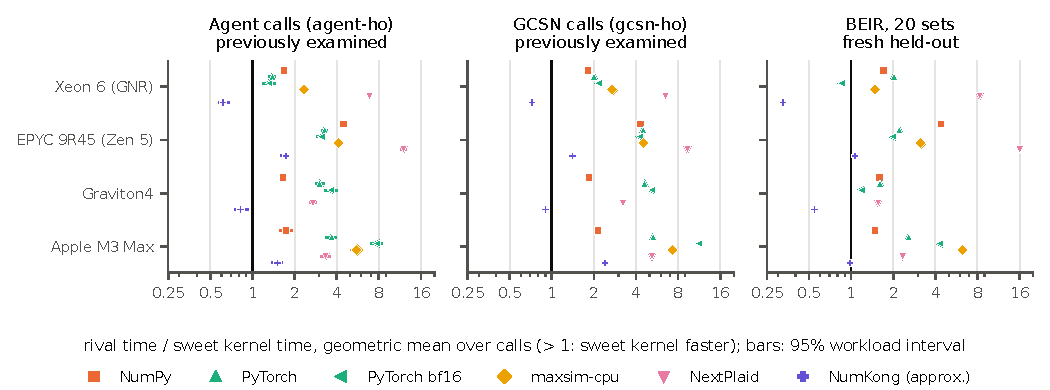
\includegraphics[width=\linewidth]{figures/ratios.pdf}
\caption{Warm speed ratios, all cores (rival time / \sweet time; above 1: \sweet faster), with the 95\% workload interval. Frozen rival configurations; NumKong shows its fastest input type. Agent and GCSN calls are previously examined; BEIR is fresh held-out.}
\label{fig:ratios}
\end{figure}

\subsection{Size sweep}
\label{sec:sweep}

Figure~\ref{fig:sweep} shows, per sweep cell, the fastest frozen exact float32 rival against \sweet.
On the cloud CPUs all 84 cells ran; the M3 Max ran \nm{sweep.m3max.cells} cells (a reduced grid of 24, decided before any result, plus 2 complete cells from before that decision).
The fastest exact rival was faster than \sweet in \nm{sweep.intel.lose} of \nm{sweep.intel.cells} cells on Intel, \nm{sweep.amd.lose} on AMD, \nm{sweep.arm.lose} on Graviton4 and \nm{sweep.m3max.lose} of \nm{sweep.m3max.cells} on the M3 Max.
The losses form bands.
On AMD, PyTorch was faster for pools of 64 to 1,024 short documents at every query length (worst cell: \nm{sweep.amd.worstcell}, \nm{sweep.amd.worst}$\times$), while \sweet was faster for smaller and larger pools.
On Intel and Graviton4, most losses are at 32 and 64 query tokens with 64 to 4,096 documents (mostly PyTorch, some NextPlaid), plus single documents with 32 or 64 query tokens (NumPy).
On the M3 Max, maxsim-cpu and PyTorch (both on Apple Accelerate, which uses the AMX matrix unit) were faster for single documents with 32 or 64 query tokens and for the largest pools.
At 8 query tokens, \sweet was faster in every cell on Intel, Graviton4 and the M3 Max.
We did not decompose the cost of a call (Section~\ref{sec:limits}), so these figures show where \sweet loses, not why.
NumKong is not in the figure; it was faster than \sweet in most sweep cells on every CPU (Section~\ref{sec:losses}).

\begin{figure}[!htbp]
\centering
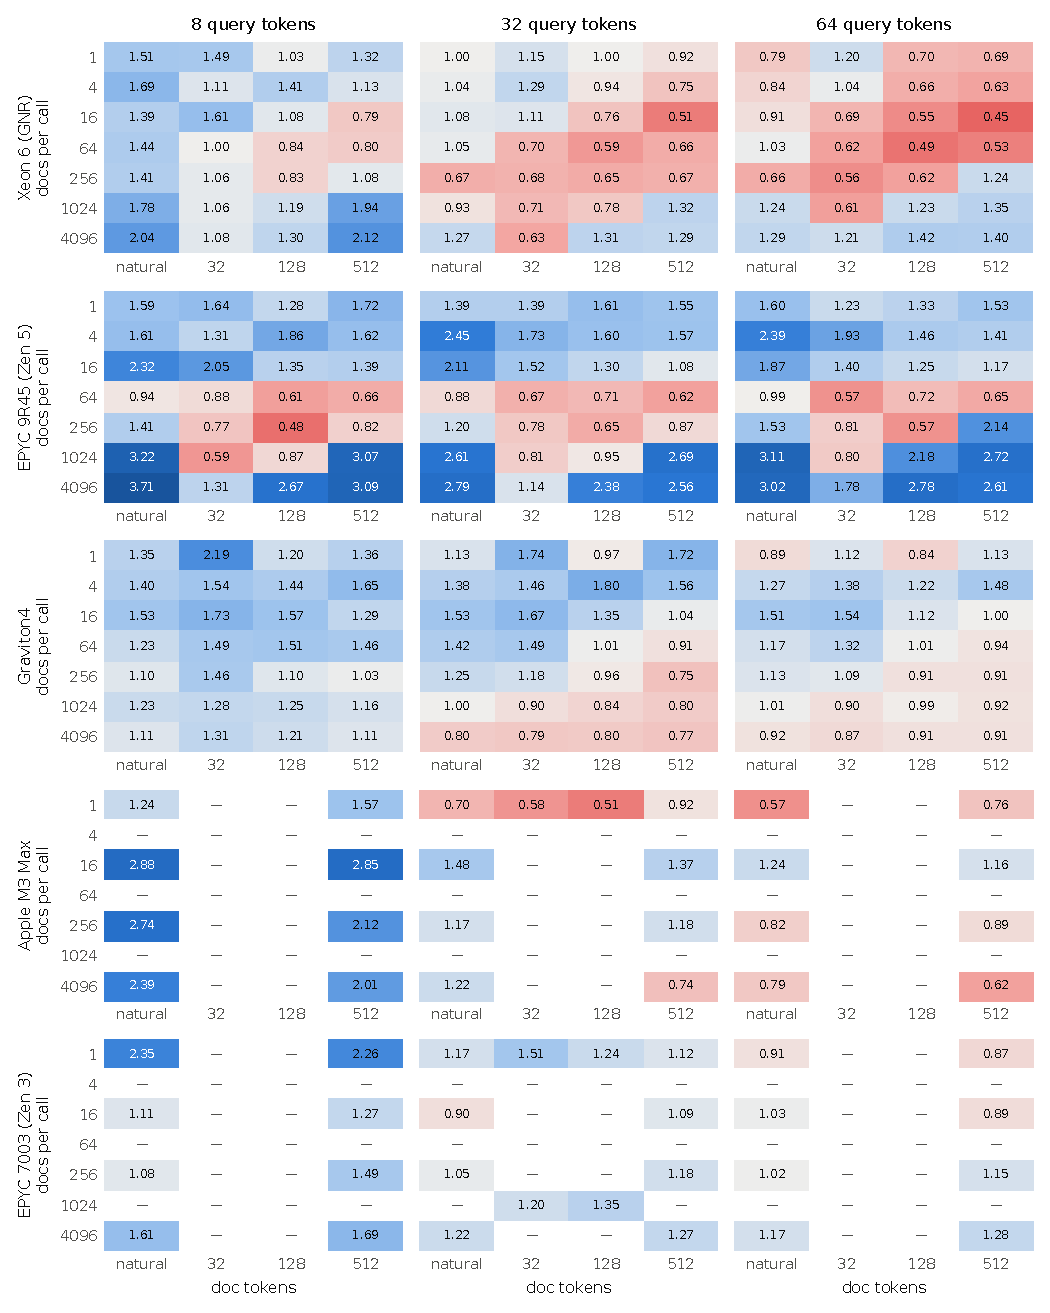
\includegraphics[width=\linewidth]{figures/sweep.pdf}
\caption{Size sweep (previously examined), warm, all cores: fastest frozen exact float32 rival / \sweet per cell (geometric mean over the cell's calls; blue: \sweet faster, red: the rival is faster; log colour scale). Rows: CPUs; columns: query tokens; inside: documents per call $\times$ tokens per document. ``--'': cell not run (reduced local grid).}
\label{fig:sweep}
\end{figure}

\subsection{Quality on BEIR: int4 against float32}
\label{sec:quality}

\paragraph{The pre-registered test.}
Before the freeze we fixed four primary comparisons (both models $\times$ both datasets, $k = 100$), the margin $\delta = 0.01$ absolute nDCG@10, and the decision rule.
For each set, ``no material loss'' holds only if on every CPU both the lower bound of the paired-bootstrap 95\% interval of (K $-$ F) is above $-\delta$ and the Holm-adjusted one-sided $p$ for $H_0$: loss $\geq \delta$ is below 0.05.
K is the kernel's own recorded scores; F scores the float32 vectors in float64 without clamp.
Table~\ref{tab:primary} gives the result.
For ColBERTv2, both sets pass on every CPU: K $-$ F is \nm{q.intel.scifact.colbertv2.diff} on SciFact and \nm{q.intel.nfcorpus.colbertv2.diff} on NFCorpus.
For answerai-colbert-small, both sets fail on every CPU: K $-$ F is \nm{q.intel.scifact.answersmall.diff} (\nm{q.intel.scifact.answersmall.rel}\%) on SciFact and \nm{q.intel.nfcorpus.answersmall.diff} (\nm{q.intel.nfcorpus.answersmall.rel}\%) on NFCorpus.
The secondary contrast (Q+c $-$ F, int4 decoded in float64 under contract S) gives the same values, because K and Q+c give the same nDCG@10 to four decimals in every cell, on every CPU and every $k$.

\begin{table}[!htbp]
\centering\scriptsize
\setlength{\tabcolsep}{3pt}
\caption{Primary non-inferiority tests (fresh held-out; $k = 100$; $\delta = 0.01$ absolute nDCG@10; paired bootstrap over queries, 10,000 resamples, seed 42; Holm over the four tests). Per CPU: lower 95\% bound of K $-$ F / Holm-adjusted $p$, and the verdict (\cmark: no material loss).}
\label{tab:primary}
\resizebox{\linewidth}{!}{%
\begin{tabular}{llrrrrr|ccccc}
\toprule
dataset & model & queries & F & K & K $-$ F & relative & Intel & AMD & Graviton4 & M3 Max & EPYC \\
\midrule
\inputtable{tables/primary.tex}
\bottomrule
\end{tabular}}
\end{table}

\paragraph{Where the loss comes from.}
Table~\ref{tab:effects} separates the score sources at $k = 100$.
The clamp has no effect (F+c = F).
The kernel's arithmetic has no effect (K = Q+c).
The whole loss enters between F+c and Q+c, that is, with the int4 storage under contract S.
The decoding error itself is the same for both models: the median relative error of a decoded token is \nm{int4diag.scifact.colbertv2.relerr} for ColBERTv2 and \nm{int4diag.scifact.answersmall.relerr} for answerai-colbert-small, and the median cosine between a token and its decoding is \nm{int4diag.scifact.colbertv2.cos} and \nm{int4diag.scifact.answersmall.cos}.
The two models differ in what contract S does with that error.
Contract S divides the decoded token by the norm of the token \emph{before} quantization, so any change of length by quantization enters the score.
Contract C on the same int4 data divides by the norm of the decoded token itself; its nDCG@10 (C-b) is \nm{nd.scifact.answersmall.Cb} on SciFact and \nm{nd.nfcorpus.answersmall.Cb} on NFCorpus, close to the float32 values of \nm{nd.scifact.answersmall.F} and \nm{nd.nfcorpus.answersmall.F}.
This analysis is post hoc and descriptive: we did not pre-register it, and we did not change or test the production rule.
It suggests that the loss is a property of the normalization in the storage format, not of int4 precision as such and not of the kernel.

\begin{table}[!htbp]
\centering\scriptsize
\setlength{\tabcolsep}{3.5pt}
\caption{nDCG@10 by score source at $k = 100$ (fresh held-out). BM25: candidate order. F: float32 vectors, float64, no clamp; F+c: with clamp; Q+c: int4 decoded in float64, contract S; K: \sweet kernel scores; C-b: contract C on float64-decoded int4; C-a: contract C on NumKong's float32 inputs; NumKong: its recorded scores (float32 input, Intel run). Post-hoc columns: C-b, C-a.}
\label{tab:effects}
\begin{tabular}{llrrrrrrrr}
\toprule
dataset & model & BM25 & F & F+c & Q+c & K & C-b & C-a & NumKong \\
\midrule
\inputtable{tables/effects.tex}
\bottomrule
\end{tabular}
\end{table}

\paragraph{NumKong's approximation.}
Contract C itself costs little against S for ColBERTv2.
NumKong's token selection costs more: on SciFact with answerai-colbert-small, its own scores give nDCG@10 \nm{nd.scifact.answersmall.NK} against \nm{nd.scifact.answersmall.Ca} for the exact value of its contract on its own inputs.
On the BEIR sets its top-ranked document agreed with the contract-S reference on only 57--58\% of calls; its bfloat16 path on the Xeon, which uses AMX, agreed on 78\% (Table~\ref{tab:correctness}).

\paragraph{The kernel across CPUs.}
The kernel's BEIR scores were bit-identical between Intel and AMD (both AVX-512) and between Graviton4 and the M3 Max (both NEON).
Between the two instruction sets, \nm{xplat.armequal.lo}--\nm{xplat.armequal.hi}\% of scores were bit-identical and the largest difference was \nm{xplat.maxabs}; the full candidate ranking was the same on at least \nm{xplat.sameranking.min}\% of calls, and nDCG@10 agreed to four decimals.
Within one CPU, the scores of all thread budgets, rounds and processes were bit-identical (2,000 result files, 48 million scores).

\subsection{Quality per latency budget}
\label{sec:budget}

A faster scorer can rerank more candidates within the same time.
Figure~\ref{fig:budget} plots nDCG@10 against the per-request p95 of the timed scoring call, one point per $k$; Table~\ref{tab:budget} reads it at two budgets.
The time covers only the scoring call: the rivals' decoding and casting run outside their timer.
At a p95 budget of 0.25\,ms, \sweet reached $k = $ \nm{budget.intel.scifact.colbertv2.0.25.ours} (Intel), \nm{budget.amd.scifact.colbertv2.0.25.ours} (AMD), \nm{budget.arm.scifact.colbertv2.0.25.ours} (Graviton4) and \nm{budget.m3max.scifact.colbertv2.0.25.ours} (M3 Max) on SciFact with ColBERTv2.
More candidates do not always help: with ColBERTv2 on SciFact, nDCG@10 is highest at $k = 25$, and with answerai-colbert-small on NFCorpus under contract S it falls as $k$ grows.
NumKong reaches $k = 200$ within 0.25\,ms on the three cloud CPUs, at the quality cost shown above.

\begin{figure}[!htbp]
\centering
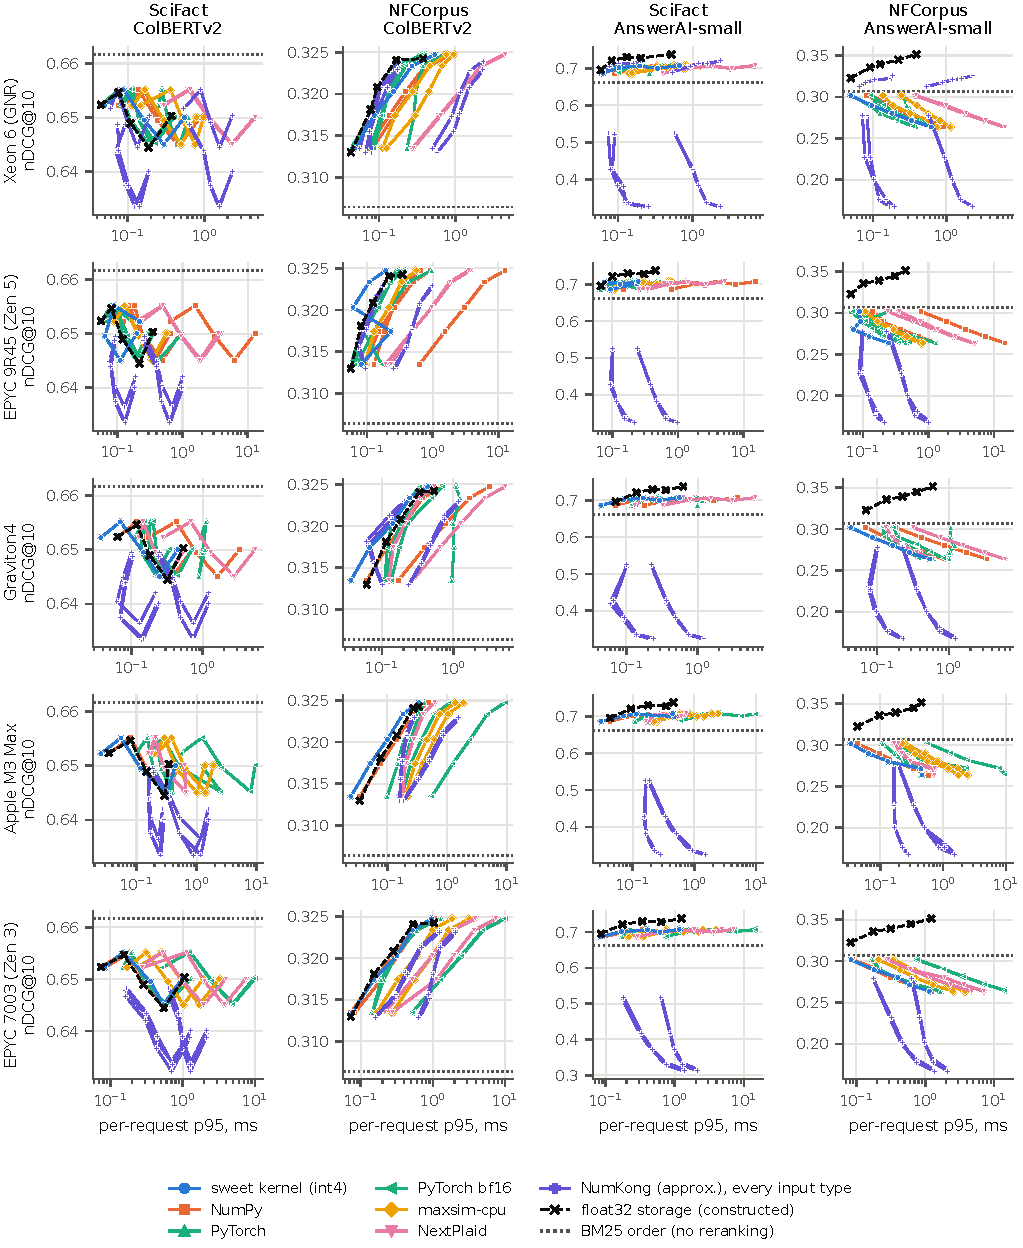
\includegraphics[width=\linewidth]{figures/budget.pdf}
\caption{Quality per latency budget (fresh held-out BEIR): nDCG@10 against per-request p95 of the timed scoring call, one point per $k \in \{10, 25, 50, 100, 200\}$. Frozen configurations; int4-self arms omitted (Table~\ref{tab:int4self}).}
\label{fig:budget}
\end{figure}

\begin{table}[!htbp]
\centering\scriptsize
\setlength{\tabcolsep}{3pt}
\caption{Largest $k$ whose per-request p95 fits the budget, with nDCG@10 at that $k$ in parentheses. ``best exact'': the frozen exact rival (any input type except int4-self) that reaches the largest $k$. NumKong: its best input type.}
\label{tab:budget}
\resizebox{\linewidth}{!}{%
\begin{tabular}{llllllll}
\toprule
& & \multicolumn{3}{c}{p95 $\leq$ 0.25\,ms} & \multicolumn{3}{c}{p95 $\leq$ 0.5\,ms} \\
CPU & set & \sweet & best exact & NumKong & \sweet & best exact & NumKong \\
\midrule
\inputtable{tables/budget.tex}
\bottomrule
\end{tabular}}
\end{table}

\subsection{Pool-parked calls (5\,ms busy gap)}
\label{sec:parked}

When other work runs for 5\,ms before each call, the worker pool of \sweet has parked and must be woken.
Table~\ref{tab:parked} shows that this changes the ranking.
NumPy was faster than \sweet on Intel (\nm{parked.intel.agent-ho.numpy.f32}$\times$ on agent calls, \nm{parked.intel.gcsn-ho.numpy.f32}$\times$ on GCSN calls, \nm{parked.intel.beir.numpy.f32}$\times$ on BEIR calls), on Graviton4 (\nm{parked.arm.agent-ho.numpy.f32}$\times$ and \nm{parked.arm.gcsn-ho.numpy.f32}$\times$) and on the M3 Max (\nm{parked.m3max.agent-ho.numpy.f32}$\times$ and \nm{parked.m3max.gcsn-ho.numpy.f32}$\times$). We did not measure why; one plausible cause is that OpenBLAS and Accelerate keep their threads awake longer than the 200\,$\mu$s spin of \sweet.
On AMD, \sweet stayed faster than every rival.
The product path calls a prewarm function when the rerank stage starts, so the pool wakes while other work runs; with it, a call took \nm{range.parked.prewarm.agent.min}--\nm{range.parked.prewarm.agent.max}$\times$ the time of the bare kernel (without prewarm) on agent calls.
On the Mac and the EPYC box, the BEIR idle-gap groups were not run (Appendix~\ref{app:deviations}).

\begin{table}[!htbp]
\centering\scriptsize
\setlength{\tabcolsep}{3pt}
\caption{Pool-parked calls (5\,ms busy gap before each call; 3 timed repetitions). Ratio = rival / \sweet kernel, both after the gap. ``prewarm'': the product path with its prewarm call; ``prod.\ path'': without it. BEIR: the 8 sets with $k \in \{25, 100\}$ (cloud CPUs only). Agent and GCSN previously examined; BEIR fresh.}
\label{tab:parked}
\begin{tabular}{llrrrrrrrrr}
\toprule
CPU & set & calls & NumPy & PyTorch & PyTorch bf16 & maxsim-cpu & NextPlaid & NumKong$^\dagger$ & prewarm & prod.\ path \\
\midrule
\inputtable{tables/parked.tex}
\bottomrule
\end{tabular}
\end{table}

\subsection{One thread}
\label{sec:single}

Table~\ref{tab:single} compares each library's frozen one-thread configuration with \sweet on one thread.
On agent and GCSN calls on the three Linux CPUs, \sweet was faster than every exact rival (the closest, NumPy, needed \nm{range.single.numpy.linux.agentgcsn.min}--\nm{range.single.numpy.linux.agentgcsn.max}$\times$ the time).
On BEIR calls (32-token queries, up to 200 candidates), a rival was faster on every CPU: NumPy on Intel (\nm{single.intel.beir.numpy.f32}$\times$) and AMD (\nm{single.amd.beir.numpy.f32}$\times$), PyTorch on Graviton4 (\nm{single.arm.beir.torch.f32}$\times$).
So the all-core advantage on BEIR calls does not come from faster arithmetic per core.
On the M3 Max, NumPy, PyTorch and maxsim-cpu call Apple Accelerate, which runs matrix products on the AMX coprocessor whatever the thread limit; their one-thread rows are therefore not one core against one core, and they were faster than \sweet on all three workloads.

\begin{table}[!htbp]
\centering\scriptsize
\setlength{\tabcolsep}{3pt}
\caption{One thread each (frozen one-thread configurations; not pinned to a core). Ratio = rival / \sweet with one thread. On the M3 Max, Accelerate-based rivals use the AMX coprocessor whatever the thread limit.}
\label{tab:single}
\begin{tabular}{llrrrrrrr}
\toprule
CPU & set & calls & NumPy & PyTorch & PyTorch bf16 & maxsim-cpu & NextPlaid & NumKong$^\dagger$ \\
\midrule
\inputtable{tables/single.tex}
\bottomrule
\end{tabular}
\end{table}

\subsection{Rivals on the same int4 storage}

When NumPy and maxsim-cpu receive the same int4 storage as \sweet and decode it inside their timed call, they were \nm{range.int4self.min}--\nm{range.int4self.max}$\times$ slower (Table~\ref{tab:int4self}).
This is the cost that the other rows leave out of the timer: in a system that stores int4, a float32 rival must decode before it scores, or keep a float32 copy (Section~\ref{sec:memory}).

\begin{table}[!htbp]
\centering\scriptsize
\caption{Rivals given the same int4 storage, decoding inside their timed call (``int4-self''). Ratio = rival / \sweet kernel, warm, all cores.}
\label{tab:int4self}
\begin{tabular}{llrr}
\toprule
CPU & set & NumPy int4-self & maxsim-cpu int4-self \\
\midrule
\inputtable{tables/int4self.tex}
\bottomrule
\end{tabular}
\end{table}

\subsection{Parallel callers}
\label{sec:conc}

In a service, several requests can score at the same time.
We ran $N \in \{1, 4, 16\}$ callers in two executors: threads in one process (the library's pool is shared), and one process per caller with a thread budget of $\max(1, \text{cores}/N)$.
\emph{Closed-loop saturation} lets each caller replay its share of a set back to back; we report throughput.
\emph{Open-loop} runs use one Poisson arrival trace per rate (seed 42; the same timestamps and call order for every arm); the rates are absolute and common to all arms on a machine: 25, 50 and 75\% of the closed-loop throughput of the slowest shortlisted rival on development data, frozen.
Their latency includes queueing.

Table~\ref{tab:conc} and Figure~\ref{fig:conc} give the results (best executor per arm).
With one caller, \sweet had \nm{range.conc.n1.min}--\nm{range.conc.n1.max}$\times$ the throughput of the best exact rival.
With 16 callers the margin shrank, and an exact rival had the higher throughput in two of eight CPU--workload pairs: NextPlaid on Graviton4 GCSN calls and NumPy on M3 Max agent calls.
NumKong had a higher throughput than \sweet at 16 callers in every pair.
At the highest common open-loop rate, the best exact rival had a lower per-request p99 than \sweet on M3 Max GCSN calls only.
During the analysis we found a defect in the harness: in closed-loop runs of the per-process executor, callers start about 50\,ms before the recorded start time, so the recorded wall time is too short.
We corrected these throughputs by adding 48.8--50\,ms (the bound follows from the 1\,ms polling of the start file) and report the lower bound; the per-request latencies need no correction (Appendix~\ref{app:deviations}).

\begin{table}[!htbp]
\centering\scriptsize
\setlength{\tabcolsep}{3pt}
\caption{Parallel callers (previously examined sets). Closed loop: \sweet throughput in thousand calls/s, and \sweet / best exact rival and \sweet / best NumKong configuration (above 1: \sweet faster; red: rival faster). Open loop: per-request p99 in ms at the highest common rate (calls/s), \sweet and the best exact rival (red: rival lower).}
\label{tab:conc}
\resizebox{\linewidth}{!}{%
\begin{tabular}{llrlrrlrrrl}
\toprule
& & \multicolumn{3}{c}{1 caller} & \multicolumn{3}{c}{16 callers} & \multicolumn{3}{c}{open loop, top rate} \\
CPU & set & \sweet & exact & NumKong & \sweet & exact & NumKong & rate & \sweet p99 & exact p99 \\
\midrule
\inputtable{tables/conc.tex}
\bottomrule
\end{tabular}}
\end{table}

\begin{figure}[!htbp]
\centering
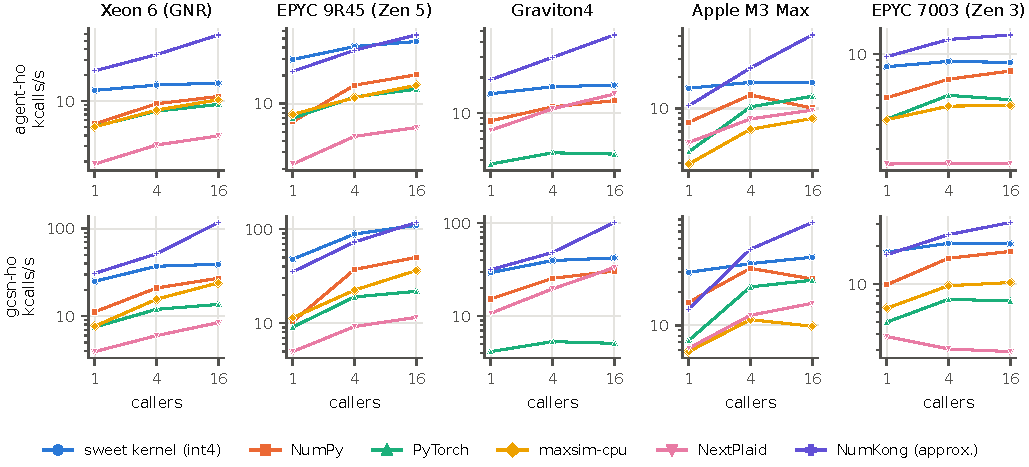
\includegraphics[width=\linewidth]{figures/conc.pdf}
\caption{Closed-loop saturation throughput against the number of callers (best executor per library; previously examined sets; log scales).}
\label{fig:conc}
\end{figure}

\subsection{Memory}
\label{sec:memory}

A separate, untimed pass per arm and set measured resident memory in a fresh process (Linux: \texttt{VmRSS}, \texttt{VmHWM} and \texttt{smaps\_rollup}; macOS: resident size from a 0.2\,ms sampler).
The allocator returned freed large blocks at once, so a later phase cannot reuse them unseen.
Table~\ref{tab:memory} reports resident bytes per stored document token (the int4 store for arms that read it, plus the arm's own prepared copy) and the peak temporary memory of the largest call.
\sweet holds \nm{mem.intel.ours.bpt} bytes per token at dimension 128 and \nm{mem.intel.ours.bpt96} at dimension 96, the size of the int4 store itself.
The float32 rivals hold their decoded copy: about 520 bytes per token for NumPy and \nm{mem.intel.torch_pad_bmm.bpt} for padded PyTorch on Intel.
The int4-self rivals hold the store and peak at about 280\,MB of temporary memory on the largest agent call.

\begin{table}[!htbp]
\centering\scriptsize
\caption{Memory on agent-ho (previously examined): resident bytes per stored document token / peak temporary memory of the largest call in MiB. Computed sizes at dimension 128: int4 76, bfloat16 256, float32 512 bytes per token.}
\label{tab:memory}
\begin{tabular}{lrrrrr}
\toprule
arm & Intel & AMD & Graviton4 & M3 Max & EPYC \\
\midrule
\inputtable{tables/memory.tex}
\bottomrule
\end{tabular}
\end{table}

\subsection{Instance-to-instance spread}
\label{sec:spread}

A replica instance of each cloud type repeated agent-ho and gcsn-ho.
Across \nm{replica.n} rival ratios, the ratio on the replica differed from the shard by a median of \nm{replica.median}\% and at most \nm{replica.maxabs}\%; no ratio changed sides of 1 (Table~\ref{tab:replica}).
The kernel's own geometric-mean latency differed by at most \nm{replica.oursmax}\%.
Each replica was a different instance in the same availability zone.
EC2 does not expose the physical host of shared-tenancy instances, so we cannot show that the hosts differed.

\begin{table}[!htbp]
\centering\scriptsize
\caption{Instance-to-instance spread: absolute relative difference of each frozen rival ratio between the shard and the replica instance (median and maximum, \%), and the change of the \sweet kernel's geometric-mean latency.}
\label{tab:replica}
\begin{tabular}{llrrrr}
\toprule
CPU & set & ratios & median \% & max \% & \sweet latency \% \\
\midrule
\inputtable{tables/replica.tex}
\bottomrule
\end{tabular}
\end{table}
